% Provide commands for drawing single modules and neural nets
% Provide commands for drawing convolution layers

% Packages
%%%%%%%%%%
\usepackage{xcolor}
\usepackage{tikz}
\usepackage{tikz-3dplot}
\usepackage[customcolors]{hf-tikz}
\usetikzlibrary{shapes,
                shadings,
                calc,
                arrows,
                backgrounds,
                colorbrewer,
                shadows.blur}
\usepackage{ifthen}
\usepackage{comment}


% Adjustable colors:
%%%%%%%%%%%%%%%%%%%%
% in case colorbrewer colors do not work
\definecolor{YlGnBu-5-1}{RGB}{255,255,204}
\definecolor{YlGnBu-5-2}{RGB}{161,218,180}
\definecolor{YlGnBu-5-3}{RGB}{65,182,196}
\definecolor{YlGnBu-5-4}{RGB}{44,127,184}
\definecolor{YlGnBu-5-5}{RGB}{37,52,148}
\definecolor{RdPu-5-1}{RGB}{254,235,226}
\definecolor{RdPu-5-2}{RGB}{251,180,185}
\definecolor{RdPu-5-3}{RGB}{247,104,161}
\definecolor{RdPu-5-4}{RGB}{197,27,138}
\definecolor{RdPu-5-5}{RGB}{122,1,119}


% module colors
\colorlet{forwardFill}{YlGnBu-5-1}
\colorlet{forwardDraw}{black}
\colorlet{backwardGradientFill}{YlGnBu-5-2}
\colorlet{backwardGradientDraw}{black}
\colorlet{backwardHessianFill}{YlGnBu-5-3}
\colorlet{backwardHessianDraw}{black}

% arrow colors
\colorlet{thickArrow}{black}
\colorlet{thickParamArrow}{black}

% - moduleFill
\colorlet{moduleFill}{black!50!white}
% - moduleFrameFill
\colorlet{moduleFrameFill}{moduleFill!50!white}

% - moduleDraw
\colorlet{moduleDraw}{black}
% - moduleFrameDraw
\colorlet{moduleFrameDraw}{moduleDraw}


% Adjustable distances:
%%%%%%%%%%%%%%%%%%%%%%%
% - \nodeMinWidth
\pgfmathsetmacro{\nodeMinWidth}{7.5}
% - \nodeMinHeight
\pgfmathsetmacro{\nodeMinHeight}{4}
% - \vNodeDistance
\pgfmathsetmacro{\vNodeDistance}{4.5}
% - \hNodeDistance
\pgfmathsetmacro{\hNodeDistance}{12.5}

% - \moduleMinHeight
\pgfmathsetmacro{\moduleMinHeight}{3*\vNodeDistance}

% - \paramArrowYShift
\pgfmathsetmacro{\paramArrowYShift}{-0.7}
% - \paramArrowSplit
\pgfmathsetmacro{\paramArrowSplit}{2}


%%%%%%%%
% Styles
%%%%%%%%
\tikzset{thickArrow/.style={
		->,
		>=stealth,
		thick,
		draw=thickArrow,
		rounded corners=1ex
	}
}

\tikzset{thickParamArrow/.style={
		thickArrow,
		draw=thickParamArrow,
	}
}


\tikzset{moduleFrame/.style={
		rounded corners=1ex,
		minimum height=\moduleMinHeight ex,
		draw=moduleFrameDraw,
		fill=moduleFrameFill,
		inner sep=0
	}
}


\tikzset{module/.style={
		rectangle,
		rounded corners=1ex,
		minimum height=\moduleMinHeight ex,
		draw=moduleDraw,
		fill=moduleFill,
		inner sep=0
	}
}


\tikzset{forward/.style={
		rectangle,
		rounded corners=1ex,
		minimum width=\nodeMinWidth ex,
		minimum height=\nodeMinHeight ex,
		draw=forwardDraw,
		fill=forwardFill
	}
}


\tikzset{backwardGradient/.style={
		rectangle,
		rounded corners=1ex,
		minimum width=\nodeMinWidth ex,
		minimum height=\nodeMinHeight ex,
		draw=backwardGradientDraw,
		fill=backwardGradientFill
	}
}


\tikzset{backwardHessian/.style={
		rectangle,
		rounded corners=1ex,
		minimum width=\nodeMinWidth ex,
		minimum height=\nodeMinHeight ex,
		draw=backwardHessianDraw,
		fill=backwardHessianFill
	}
}


%%%%%%%%%%%%%%%
% Draw commands
%%%%%%%%%%%%%%%
\newcommand{\drawMessages}[3]{
	% input
	\ifthenelse{\equal{#1}{ }}{}{
        \node (input)
            [forward]
            { #1 };
	}
	% gradient
	\ifthenelse{\equal{#2}{ }}{}{	
	\node (inputGradient)
		[backwardGradient,
		below of=input,
		node distance=\vNodeDistance ex]
		{ #2 };	
	}
	% hessian
	% phantom for alignment
	\ifthenelse{\equal{#3}{ }}{
        \phantom{
            \node (inputHessian)
            [backwardHessian,
            below of=input,
            node distance=2*\vNodeDistance ex]
            { #3 };		
        }	
	}{	
        \node (inputHessian)
            [backwardHessian,
            below of=input,
            node distance=2*\vNodeDistance ex]
            { #3 };
	}	
}


\newcommand{\drawMessagesWithArrows}[4]{
	\drawMessages{#1}{#2}{#3}
	\begin{pgfonlayer}{background}
        % arrows in background
        \ifthenelse{\equal{#1}{ }}{}{
            \draw [thickArrow]
                ($(input)+(-{#4 ex/2},0)$) to ++(#4 ex, 0);
        }
        \ifthenelse{\equal{#2}{ }}{}{
            \draw [thickArrow, <-]
                ($(inputGradient)+(-{#4 ex/2},0)$) to ++(#4 ex, 0);
        }
        \ifthenelse{\equal{#3}{ }}{}{
            \draw [thickArrow, <-]
                ($(inputHessian)+(-{#4 ex/2},0)$) to ++(#4 ex, 0);
        }	
	\end{pgfonlayer}
}


\newcommand{\drawParamsWithArrows}[3]{
	\drawMessages{#1}{#2}{#3}
	% arrows in background
	\ifthenelse{\equal{#1}{ }}{}{
		\coordinate (arrowParam) at
             ($(inputHessian.south east)+(3*\paramArrowSplit ex, \paramArrowYShift ex)$);
		\draw [thickParamArrow] (input.east) -| (arrowParam);
	}
	\ifthenelse{\equal{#2}{ }}{}{
		\coordinate (arrowGradient) at
             ($(inputHessian.south east)+(2*\paramArrowSplit ex, \paramArrowYShift ex)$);
		\draw [thickParamArrow] (arrowGradient) |- (inputGradient.east);
	}
	\ifthenelse{\equal{#3}{ }}{}{
		\coordinate (arrowHessian) at
            ($(inputHessian.south east)+(\paramArrowSplit ex, \paramArrowYShift ex)$);
		\draw [thickParamArrow] (arrowHessian) |- (inputHessian.east);
	}	
}


\newcommand{\drawModuleWithParams}[5]{			
	\node (moduleFrame) [moduleFrame] {
		\tikz{
			\node (module)
                [module, minimum width=#2 ex]
                { #1 };
			\node (moduleParams)
                [anchor=south]
                at (module.north)
                {\tikz \drawParamsWithArrows{#3}{#4}{#5};};
		}
	};			
}

\newcommand{\drawModuleNoParams}[2]{			
	\node (module) [module, minimum width=#2 ex] { #1 };			
}

%%%%%%%%%%
% Examples
%%%%%%%%%%
\begin{comment}
    \begin{tikzpicture}
        \node (a)
            {\tikz \drawMessages{a}{b}{c};};
        \node (b)
            [right of=a]
            {\tikz \drawMessages{a}{ }{ };};
        \node (c)
            [right of=b]
            {\tikz \drawMessages{a}{ }{c};};
        \node (d)
            [right of=c, node distance=15ex]
            {\tikz \drawMessagesWithArrows{a}{ }{c}{\hNodeDistance};};
        \node (e)
            [right of=d, node distance=15ex]
            {\tikz \drawParamsWithArrows{a}{b}{c}{\hNodeDistance};};
        \node (f)
            [right of=e, node distance=20ex]
            {\tikz \drawModuleWithParams{f(x)}{14}{b}{c}{d};};
        \node (g)
            [right of=f, node distance=20ex]
            {\tikz \drawModuleNoParams{f(x)}{10};};	
    \end{tikzpicture}
\end{comment}
	

%%%%%%%%%%%%%%%%%%%%%%%%
% CONVOLUTION COMMANDS %
%%%%%%%%%%%%%%%%%%%%%%%%

% Draw a 2d tiled image with shaded background
% Parameters:
% 1) Depth coordinate
% 2) Image width
% 3) Image height
% 4) fillcolor
% 5) name 
% Cells are available by coordinates (name-x-y)
\newcommand{\drawGrid}[5]{
  \foreach \i in {1, ..., #2}{
    \foreach \j in {#3, ..., 1}{
      \draw[canvas is yz plane at x=#1,
            transform shape,
            draw=black,
            fill=#4,
            drop shadow=black]
      (\i,\j) rectangle ++(-1, -1) coordinate [pos=0.5] (#5-\i-\j);
    }
}
}

% Draw a 2d tiled image without shaded background
% Additional parameters
% 6) Start position i
% 7) Start position j
\newcommand{\drawGridNoShadow}[7]{
  \foreach \i in {#6, ..., #2}{
    \foreach \j in {#3, ..., #7}{
      \draw[canvas is yz plane at x=#1,
            transform shape,
            draw=black,
            fill=#4]
      (\i,\j) rectangle ++(-1, -1) coordinate [pos=0.5] (#5-\i-\j);
    }
}
}

% Insert text at position i, j
% Parameters:
% 1) Depth coordinate
% 2) Index i
% 3) Index j
% 4) Text
\newcommand{\drawGridTextLabel}[4]{
  \node[canvas is yz plane at x=#1,
        transform shape] at ($(0, -0.5,-0.5) + (0, #2, #3)$) {#4};
}


%%%%%%%%%%%%%%%%%%%%%%%%
% CONVOLUTION EXAMPLES %
%%%%%%%%%%%%%%%%%%%%%%%%
\begin{comment}
  \tdplotsetmaincoords{85}{110}

  \begin{tikzpicture}[scale=1,tdplot_main_coords]
    \drawGrid{0}{3}{3}{blue!50!white}{channelBlue};
    \drawGridNoShadow{0}{3}{3}{blue}{channelBlue}{2}{2};
    \drawGridTextLabel{0}{3}{3}{b};

    \drawGrid{1}{2}{2}{green!50!white}{greenChannel};
    \drawGridTextLabel{1}{2}{2}{g};

    \drawGrid{2}{1}{1}{red!50!white}{redChannel};
    \drawGridTextLabel{2}{1}{1}{r};
  \end{tikzpicture}
\end{comment}


%%%%%%%%%%%%%%%%%%%%%%%%%%%%%%%%%%%%%%%%%
% COMMANDS FOR CONVOLUTION ILLUSTRATION %
%%%%%%%%%%%%%%%%%%%%%%%%%%%%%%%%%%%%%%%%%
% channel colors
\colorlet{foregroundChannel}{YlGnBu-5-2}
\colorlet{centerChannel}{YlGnBu-5-3}
\colorlet{backgroundChannel}{YlGnBu-5-4}
% output colors
\colorlet{foregroundOutput}{RdPu-5-2}
\colorlet{backgroundOutput}{RdPu-5-4}


% matrix filling styles
\tikzset{style inputBackground/.style={
    set fill color=backgroundChannel,
    set border color=black,
    thin,
    rounded corners=0pt
  },
  style inputCenter/.style={
    set fill color=centerChannel,
    set border color=black,
    thin,
    rounded corners=0pt
  },
  style inputForeground/.style={
    set fill color=foregroundChannel,
    set border color=black,
    thin,
    rounded corners=0pt
  },
  style inputBackgroundLight/.style={
    set fill color=backgroundChannel!50!white,
    set border color=black,
    thin,
    rounded corners=0pt
  },
  style inputCenterLight/.style={
    set fill color=centerChannel!50!white,
    set border color=black,
    thin,
    rounded corners=0pt
  },
  style inputForegroundLight/.style={
    set fill color=foregroundChannel!50!white,
    set border color=black,
    thin,
    rounded corners=0pt
  },
  horizontal/.style={
    above left offset={-0.15,0.31},
    below right offset={0.15,-0.125},
    #1
  },
  vertical/.style={
    above left offset={-0.1,0.3},
    below right offset={0.15,-0.15},
    #1
  },
  style outputForeground/.style={
    set fill color=foregroundOutput,
    set border color=black,
    thin,
    rounded corners=0pt
  },
   style outputBackground/.style={
    set fill color=backgroundOutput,
    set border color=black,
    thin,
    rounded corners=0pt
  },
   style outputForegroundLight/.style={
    set fill color=foregroundOutput!50!white,
    set border color=black,
    thin,
    rounded corners=0pt
  },
   style outputBackgroundLight/.style={
    set fill color=backgroundOutput!50!white,
    set border color=black,
    thin,
    rounded corners=0pt
  },
}


\newcommand{\setCoordinates}{
  \tdplotsetmaincoords{85}{110}
}

% Requires depth coordinate
\newcommand{\drawInputBackgroundChannel}[1]{
    % background image channel
    \drawGrid{#1}{3}{3}{backgroundChannel!50!white}{channelA}
    \drawGridNoShadow{#1}{2}{2}{backgroundChannel}{channelA}{1}{3}
    %% numbers (golden ratio)
    \drawGridTextLabel{#1}{1}{3}{1}
    \drawGridTextLabel{#1}{2}{3}{6}
    \drawGridTextLabel{#1}{3}{3}{1}
    \drawGridTextLabel{#1}{1}{2}{8}
    \drawGridTextLabel{#1}{2}{2}{0}
    \drawGridTextLabel{#1}{3}{2}{3}
    \drawGridTextLabel{#1}{1}{1}{3}
    \drawGridTextLabel{#1}{2}{1}{9}
    \drawGridTextLabel{#1}{3}{1}{8}
}

\newcommand{\drawInputCenterChannel}[1]{
    % center image channel
    \drawGrid{#1}{3}{3}{centerChannel!50!white}{channelB}
    \drawGridNoShadow{#1}{2}{2}{centerChannel}{channelB}{1}{3}
    %% numbers (Euler constant)
    \drawGridTextLabel{#1}{1}{3}{2}
    \drawGridTextLabel{#1}{2}{3}{7}
    \drawGridTextLabel{#1}{3}{3}{1}
    \drawGridTextLabel{#1}{1}{2}{8}
    \drawGridTextLabel{#1}{2}{2}{2}
    \drawGridTextLabel{#1}{3}{2}{8}
    \drawGridTextLabel{#1}{1}{1}{1}
    \drawGridTextLabel{#1}{2}{1}{8}
    \drawGridTextLabel{#1}{3}{1}{2}
}

\newcommand{\drawInputForegroundChannel}[1]{
    % foreground image channel
    \drawGrid{#1}{3}{3}{foregroundChannel!50!white}{channelC}
    \drawGridNoShadow{#1}{2}{2}{foregroundChannel}{channelC}{1}{3}
    %% numbers (pi)
    \drawGridTextLabel{#1}{1}{3}{3}
    \drawGridTextLabel{#1}{2}{3}{1}
    \drawGridTextLabel{#1}{3}{3}{4}
    \drawGridTextLabel{#1}{1}{2}{1}
    \drawGridTextLabel{#1}{2}{2}{5}
    \drawGridTextLabel{#1}{3}{2}{9}
    \drawGridTextLabel{#1}{1}{1}{2}
    \drawGridTextLabel{#1}{2}{1}{6}
    \drawGridTextLabel{#1}{3}{1}{5}
}

\newcommand{\drawInputTensor}{
  \setCoordinates
  \begin{tikzpicture}[tdplot_main_coords]
    % 1. background image channel
    \drawInputBackgroundChannel{0}
    % 2. center image channel
    \drawInputCenterChannel{1}
    % 3. foreground image channel
    \drawInputForegroundChannel{2}
 \end{tikzpicture}
}

\newcommand{\drawInputTensorExpanded}{
  \setCoordinates
  \begin{tikzpicture}[tdplot_main_coords]
    % 1. background image channel
    \begin{scope}[yshift=0]
      \drawInputBackgroundChannel{0}
    \end{scope}
    % 2. center image channel
    \begin{scope}[yshift=100]
      \drawInputCenterChannel{0}
    \end{scope}
    % 3. foreground image channel
    \begin{scope}[yshift=200]
      \drawInputForegroundChannel{0}
    \end{scope}
 \end{tikzpicture}
}

\newcommand{\drawKernelOneOne}[1]{
    % Kernel 1, 1
    \drawGrid{#1}{2}{2}{backgroundChannel}{kernelA};
    % numbers
    \drawGridTextLabel{#1}{1}{2}{3}
    \drawGridTextLabel{#1}{2}{2}{5}
    \drawGridTextLabel{#1}{1}{1}{8}
    \drawGridTextLabel{#1}{2}{1}{-9}
}

\newcommand{\drawKernelOneTwo}[1]{
    % Kernel 1, 2
    \drawGrid{#1}{2}{2}{centerChannel}{kernelB};
    % numbers
    \drawGridTextLabel{#1}{1}{2}{-8}
    \drawGridTextLabel{#1}{2}{2}{-4}
    \drawGridTextLabel{#1}{1}{1}{-5}
    \drawGridTextLabel{#1}{2}{1}{9}
}

\newcommand{\drawKernelOneThree}[1]{
    % Kernel 1, 3
    \drawGrid{#1}{2}{2}{foregroundChannel}{kernelC};
    % numbers
    \drawGridTextLabel{#1}{1}{2}{8}
    \drawGridTextLabel{#1}{2}{2}{7}
    \drawGridTextLabel{#1}{1}{1}{-4}
    \drawGridTextLabel{#1}{2}{1}{-9}
}

\newcommand{\drawKernelTwoOne}[1]{
    % Kernel 2, 1
    \drawGrid{#1}{2}{2}{backgroundChannel}{kernelA};
    % numbers
    \drawGridTextLabel{#1}{1}{2}{7}
    \drawGridTextLabel{#1}{2}{2}{9}
    \drawGridTextLabel{#1}{1}{1}{-3}
    \drawGridTextLabel{#1}{2}{1}{2}
}

\newcommand{\drawKernelTwoTwo}[1]{
    % Kernel 2, 2
    \drawGrid{#1}{2}{2}{centerChannel}{kernelB};
    % numbers
    \drawGridTextLabel{#1}{1}{2}{0}
    \drawGridTextLabel{#1}{2}{2}{-4}
    \drawGridTextLabel{#1}{1}{1}{5}
    \drawGridTextLabel{#1}{2}{1}{2}
}

\newcommand{\drawKernelTwoThree}[1]{
    % Kernel 2, 3
    \drawGrid{#1}{2}{2}{foregroundChannel}{kernelC};
    % numbers
    \drawGridTextLabel{#1}{1}{2}{8}
    \drawGridTextLabel{#1}{2}{2}{-9}
    \drawGridTextLabel{#1}{1}{1}{4}
    \drawGridTextLabel{#1}{2}{1}{-8}
}

\newcommand{\drawKernelOne}{
  \setCoordinates
  \begin{tikzpicture}[tdplot_main_coords]
    \drawKernelOneOne{0}
    \drawKernelOneTwo{1}
    \drawKernelOneThree{2}
  \end{tikzpicture}
}

\newcommand{\drawKernelTwo}{
  \setCoordinates
  \begin{tikzpicture}[tdplot_main_coords]
    \drawKernelTwoOne{0}
    \drawKernelTwoTwo{1}
    \drawKernelTwoThree{2}
  \end{tikzpicture}
}

\newcommand{\drawKernelOneExpanded}{
  \setCoordinates
  \begin{tikzpicture}[tdplot_main_coords]
    % 1. Kernel 1, 1
    \begin{scope}[yshift=0]
      \drawKernelOneOne{0}
    \end{scope}
    % 2. Kernel 1, 2
    \begin{scope}[yshift=70]
      \drawKernelOneTwo{0}
    \end{scope}
    % 3. Kernel 1, 3
    \begin{scope}[yshift=140]
      \drawKernelOneThree{0}
    \end{scope}
 \end{tikzpicture}
}

\newcommand{\drawKernelTwoExpanded}{
  \setCoordinates
  \begin{tikzpicture}[tdplot_main_coords]
    % 1. Kernel 2, 1
    \begin{scope}[yshift=0]
      \drawKernelTwoOne{0}
    \end{scope}
    % 2. Kernel 2, 2
    \begin{scope}[yshift=70]
      \drawKernelTwoTwo{0}
    \end{scope}
    % 3. Kernel 2, 3
    \begin{scope}[yshift=140]
      \drawKernelTwoThree{0}
    \end{scope}
 \end{tikzpicture}
}

\newcommand{\drawOutputBackground}[1]{
    % Output image background
    \drawGrid{#1}{2}{2}{backgroundOutput!50!white}{channelA};
    \drawGridNoShadow{#1}{1}{2}{backgroundOutput}{channelA}{1}{2};
    % numbers
    \drawGridTextLabel{#1}{1}{2}{32}
    \drawGridTextLabel{#1}{2}{2}{-1}
    \drawGridTextLabel{#1}{1}{1}{1}
    \drawGridTextLabel{#1}{2}{1}{-29}
}

\newcommand{\drawOutputForeground}[1]{
    % Output image foreground
    \drawGrid{#1}{2}{2}{foregroundOutput!50!white}{channelB};
    \drawGridNoShadow{#1}{1}{2}{foregroundOutput}{channelB}{1}{2};
    % numbers
    \drawGridTextLabel{#1}{1}{2}{13}
    \drawGridTextLabel{#1}{2}{2}{-67}
    \drawGridTextLabel{#1}{1}{1}{-57}
    \drawGridTextLabel{#1}{2}{1}{-21}
}

\newcommand{\drawOutputTensor}{
  \setCoordinates
  \begin{tikzpicture}[tdplot_main_coords]
    \drawOutputBackground{0}
    \drawOutputForeground{1}
 \end{tikzpicture}
}


\newcommand{\drawOutputTensorExpanded}{
  \setCoordinates
  \begin{tikzpicture}[tdplot_main_coords]
    % 1. background output image
    \begin{scope}[yshift=0]
      \drawOutputBackground{0}
    \end{scope}
    % 2. foreground output image
    \begin{scope}[yshift=70]
      \drawOutputForeground{0}
    \end{scope}
 \end{tikzpicture}
}

\newcommand{\drawInputMatrix}{
  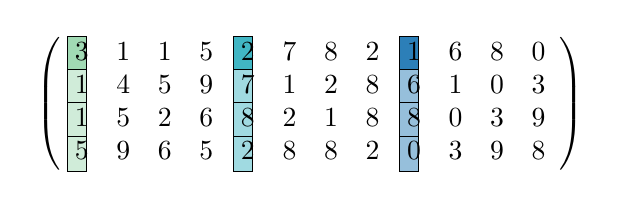
\begin{tikzpicture}
    \node {
      $\left(\begin{array}{rrrrrrrrrrrr}
               \tikzmarkin[vertical=style inputForeground]{row1col1} 3 & 1 & 1 & 5 \tikzmarkend{row1col1} & \tikzmarkin[vertical=style inputCenter]{row1col2} 2 & 7 & 8 & 2 \tikzmarkend{row1col2} & \tikzmarkin[vertical=style inputBackground]{row1col3} 1 & 6 & 8 & 0 \tikzmarkend{row1col3} \\
               \tikzmarkin[vertical=style inputForegroundLight]{row2col1} 1 & 4 & 5 & 9 \tikzmarkend{row2col1} & \tikzmarkin[vertical=style inputCenterLight]{row2col2} 7 & 1 & 2 & 8 \tikzmarkend{row2col2} & \tikzmarkin[vertical=style inputBackgroundLight]{row2col3} 6 & 1 & 0 & 3 \tikzmarkend{row2col3} \\
               \tikzmarkin[vertical=style inputForegroundLight]{row2col1} 1 & 5 & 2 & 6 \tikzmarkend{row2col1} & \tikzmarkin[vertical=style inputCenterLight]{row2col2} 8 & 2 & 1 & 8 \tikzmarkend{row2col2} & \tikzmarkin[vertical=style inputBackgroundLight]{row2col3} 8 & 0 & 3 & 9 \tikzmarkend{row2col3} \\
               \tikzmarkin[vertical=style inputForegroundLight]{row2col1} 5 & 9 & 6 & 5 \tikzmarkend{row2col1} & \tikzmarkin[vertical=style inputCenterLight]{row2col2} 2 & 8 & 8 & 2 \tikzmarkend{row2col2} & \tikzmarkin[vertical=style inputBackgroundLight]{row2col3} 0 & 3 & 9 & 8 \tikzmarkend{row2col3} \\
  \end{array}\right)
$
};
 \end{tikzpicture}
}

\newcommand{\drawKernelMatrix}{
  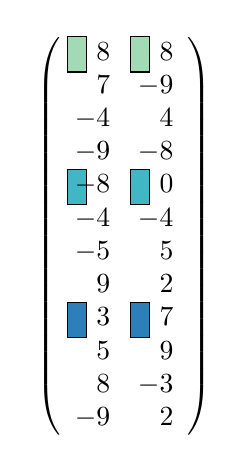
\begin{tikzpicture}
    \node {
      $\left(\begin{array}{rr}
               \tikzmarkin[vertical=style inputForeground]{krow1col1}\phantom{-}8 & \tikzmarkin[vertical=style inputForeground]{krow1col2} \phantom{-}8
               \\
               7 & -9
               \\
               -4 & 4
               \\
               -9 \tikzmarkend{krow1col1} & -8 \tikzmarkend{krow1col2}
               \\
               \tikzmarkin[vertical=style inputCenter]{krow2col1} \;\!\!\!-\;\!\!\!8 & \tikzmarkin[vertical=style inputCenter]{krow2col2} \phantom{-}0
               \\
               -4 & -4
               \\
               -5 & 5
               \\
               9 \tikzmarkend{krow2col1} & 2 \tikzmarkend{krow2col2}
               \\
               \tikzmarkin[vertical=style inputBackground]{krow3col1} \phantom{-}3 & \tikzmarkin[vertical=style inputBackground]{krow3col2} \phantom{-}7
               \\
               5 & 9
               \\
               8 & -3
               \\
               -9 \tikzmarkend{krow3col1} & 2 \tikzmarkend{krow3col2}
  \end{array}\right)
$
};
 \end{tikzpicture}
}

\newcommand{\drawOutputMatrix}{
  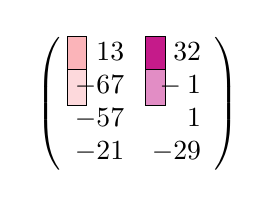
\begin{tikzpicture}
    \node {
      $\left(\begin{array}{rr}
               \tikzmarkin[vertical=style outputForeground]{orow1col1}\phantom{\;\,\,\,}13 \tikzmarkend{orow1col1} & \tikzmarkin[vertical=style outputBackground]{orow1col2} \phantom{\,\;\;}32 \tikzmarkend{orow1col2}
               \\
               \tikzmarkin[vertical=style outputForegroundLight]{orow2col1} \;\!\!\!-\;\!\!\!67 & \tikzmarkin[vertical=style outputBackgroundLight]{orow2col2} -1
               \\
               -57 & 1
               \\
               -21 \tikzmarkend{orow2col1} & -29 \tikzmarkend{orow2col2}
 \end{array}\right)
$
};
 \end{tikzpicture}
}

\newlength{\figwidth}
\newlength{\figheight}
\setlength{\figwidth}{0.9\textwidth}
\setlength{\figheight}{0.6\figwidth}

% pgfplots style
\pgfkeys{/pgfplots/HBPoriginal/.style={
    enlarge x limits = 0.,
    enlarge y limits = 0.02,
    width=\figwidth,
    height=\figheight,
    grid=major,
    grid style = {dashed},
    every axis plot/.append style={line width = 1.5pt},
    tick pos = left,
    xtick align = inside,
    ytick align = inside,
    xmajorticks = true,
    ymajorticks = true,
    ylabel near ticks,
    xlabel near ticks,
    xticklabel style = {font = \footnotesize},
    xlabel style = {font = \footnotesize},
    axis line style = {black},
    yticklabel style = {font = \footnotesize},
    ylabel style = {font = \footnotesize},
    title style = {font = \footnotesize},
    grid = major,
    grid style = {dashed},
    legend cell align = left,
    legend style = {
      fill opacity = 0.7,
      text opacity = 1,
      font = \footnotesize,
    },
  }
}

\pgfkeys{/pgfplots/HBPnolegend/.style={
    legend style = {
      fill opacity = 0.0,
      text opacity = 0.0,
      draw opacity = 0.0,
      font = \footnotesize,
    },
  }
}

\pgfkeys{/pgfplots/HBPnox/.style={
    xlabel style={opacity=0},
    xticklabel style={opacity=0, yshift=3ex},
  }
}

\newcommand{\HBPresetPGFStyle}{
  \pgfkeys{/pgfplots/mystyle/.style={
      HBPoriginal
    }}
}
\HBPresetPGFStyle

\usepackage{preamble/backpack-plotting}

% how the best runs are defined
\newcommand{\bestStrategy}{final}
\newcommand{\bestMetricType}{valid}
\newcommand{\bestMetric}{accuracies}

%%% Local Variables:
%%% mode: latex
%%% TeX-master: "../thesis"
%%% End:
